\section{Choisir la distribution des postes clients}\subsection{Information}
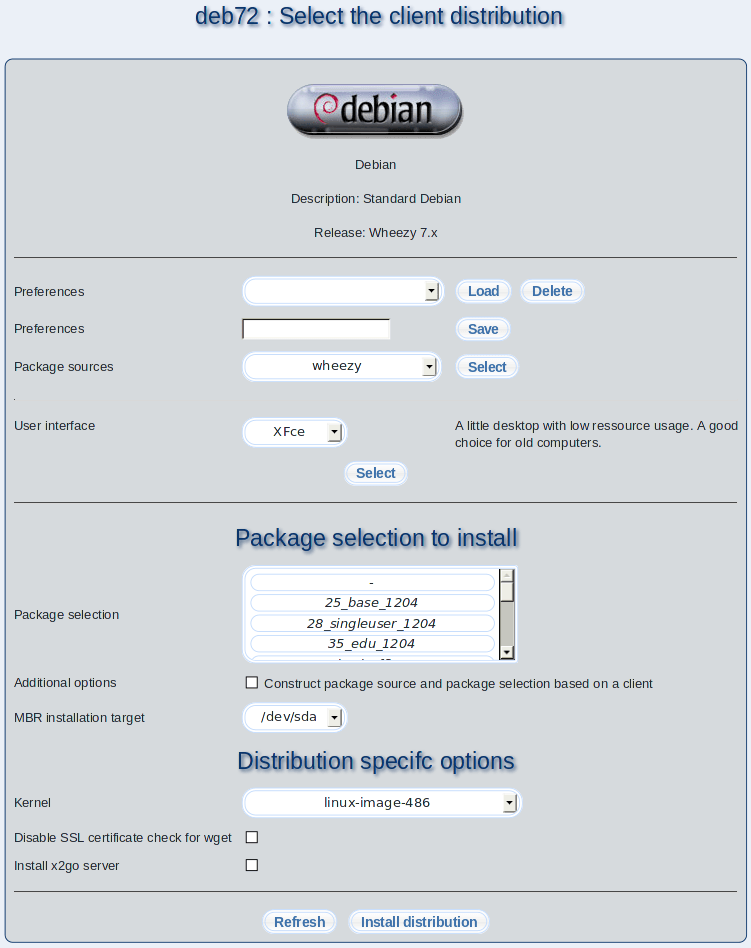
\includegraphics[scale=0.4]{/mdk/doc/manual/screenshots/fr/client_distr.png} \\
Une distribution est une collection de paquets de logiciel diff\'erents qui est vendue sur des mediums diff\'erents (CD, DVD, internet). Il y a aussi des distributions libres qu'on peut t\'el\'echarger gratuitement de l'internet. Par exemple, il y a  Debian. Les distributions diff\`erent seulement dans les programmes d'installation employ\'es et l'interface graphique du bureau. Dans la plupart des cas, le choix d'une distribution est seulement une question de go\^ut. Pour que m23 soutienne des distributions de clients diff\'erents, il y a ce dialogue.\\
\begin{itemize}
	\item \textbf{Charger des pr\'ef\'erences}: S\'electionnez une pr\'ef\'erence d\'ej\`a enregistr\'ee et cliquez sur \textit{$\ll$Charger$\gg$}.\\
	\item \textbf{Effacer des pr\'ef\'erences}: Vous pouvez effacer une pr\'ef\'erence s\'electionn\'ee en cliquant sur \textit{$\ll$Effacer$\gg$}.\\
	\item \textbf{Enregistrer des pr\'ef\'erences}: Vous pouvez enregistrer les pr\'ef\'erences actuelles en entrant un nom et cliquant sur \textit{$\ll$Enregistrer$\gg$}.\\
	\item  \textbf{Sources de paquets}: D'abord, vous devez s\'electionner une source de paquets que vous avez cr\'e\'ee sous \textit{$\ll$Paquets$\gg$} et \textit{$\ll$Sources de paquets$\gg$}. En choisissant les sources des paquets, la distribution, le release et les interfaces grafiques disponibles seront fix\'es en m\^eme temps. Pour cela, cliquez sur \textit{$\ll$Choisir$\gg$}. Puis, le logo de la distribution avec une d\'escription courte sera affich\'e en haut.\\
	\item  \textbf{Interface graphique}: En dependance de la source de paquets, vous pouvez choisir entre des interfaces graphiques diff\'erents. Comme alternative, il y a le mode de texte (textmode) pour l'installation d'un serveur qui n'a pas besoin d'un interface graphique.\\
	\item \textbf{Combinaison de paquets}: Ici, vous pouvez s\'electionner une combinaison de paquets, qui sera install\'ee au m\^eme temps que le syst\`eme d'exploitation.\\
	\item \textbf{Lieu de l'installation du MBR}: Le programme m23 essaie de d\'etecter le premier disque dur automatiquement pour y installer le chargeur d'amor\c{c}age. Si vous voudriez utiliser un disque dur diff\'erent, vous pouvez le choisir ici. Prenez en compte que ceci doit \^etre le disque dur qui sera utilis\'e pour l'amor\c{c}age par le BIOS.\\
	\item  \textbf{Configurations sp�cifiques pour la distribution}: Toute distribution peut d\'efinir une multitude d'options qui seront utilis\'e pour l'installation de cette distribution.\\
\end{itemize}
Pour commencer avec l'installation, cliquez sur \textit{$\ll$Installer la distribution$\gg$} \`a la fin.\\
\subsection{En ce qui concerne les fichiers image}
S\'electionnez la liste de sources de paquets \textit{$\ll$imaging$\gg$} pour l'installation des fichiers image.\\
En plus, vous avez le choix, si vous voudriez installer le MBR (Master Boot Record) \`a partir d'un fichier cr\'ee auparavant ou le MBR g\'en\'erique de m23, qui peut amorcer des partitions amor\c{c}ables. Pour ceci, choisissez sous \textit{$\ll$Installer un MBR � partir d'un image ou installer un MBR g�n�rique.$\gg$} entre le nom du fichier ou \textit{$\ll$MBR g�n�rique$\gg$}.\\
\subsection{Information suppl\'ementaire:}
Si vous enregistrez une pr\'eference sous le m\^eme nom sous lequel vous avez d\'ej\`a enregistr\'e des pr\'eferences pour un client, ces pr\'eferences seront ajout\'e \`a la distribution. Les configurations de la distribution seront remplac\'ees en ce cas.\\
